\documentclass[numbering=fraction]{beamer}

\usepackage[utf8]{inputenc}
\usepackage[T1]{fontenc}
\usepackage[french]{babel}
\usepackage{blindtext}
\usepackage{tikzsymbols}
\usepackage{graphicx}
\usepackage{wrapfig}
\usepackage{bookman}

\usetheme[progressbar=frametitle]{metropolis}

%Define colors
\definecolor{wuppergreen}{RGB}{85, 171, 38}
\definecolor{background}{RGB}{255,255,255}

%Adding logo to title page
\titlegraphic{\raggedleft 
\includegraphics[width=3cm]{UNamur.png}}

%Adjust color theme
\setbeamercolor{frametitle}{bg=wuppergreen}
\setbeamercolor{title separator}{fg=wuppergreen}
\setbeamercolor{footline}{fg=gray}
\setbeamercolor{progress bar}{fg=black}

\graphicspath{ {./images/}}


%Adding footer
\setbeamertemplate{frame footer}{\insertshortauthor~(\insertshortinstitute)}

%Set parameters for title page
\title{PIMS : Sprint Review 2}
\author[PIMS]{Luis Dierick \and Gaillard Matthys \and Bouncer Yassine \and Fundu Olivier \and Anderson Rosny }
\institute{Université de Namur}
\date{\today}

\begin{document}

\begin{frame}[plain]{}
    \maketitle
\end{frame}

\begin{frame}{Table des matières}
    \tableofcontents
\end{frame}
\section{Rappel et objectifs}
\begin{frame}{Rappel et objectifs}
    \begin{enumerate}
        \item Objectif : Développement d'une plateforme de gestion des mémoires à l'aide de moodle.
        \item Elément à produire lors de ce sprint
        \begin{enumerate}
            \item Définition des rôles.
            \item Création d'un dictionnaire des défintions des termes.
            \item Mockups de l'interface de la plateforme.
        \end{enumerate}
    \end{enumerate}
\end{frame}
\section{Rôles}
\begin{frame}{Rôles}
    \begin{enumerate}
        \item \textbf{\textit{Définitions}} de 4 rôles
        \begin{enumerate}
            \item \textbf{Administrateur} : Gestion de la plateforme.
            \item \textbf{Professeur} : Gestion du cours. Définition des modalités.
            \item \textbf{Etudiant} : Choisi le sujet rend des délivrables.
            \item \textbf{Superviseur} : Encadrement des étudiants dont il est le référent.
        \end{enumerate}
    \end{enumerate}
\end{frame}
\section{Dictionnaire}
\begin{frame}{Dictionnaire}
    \begin{columns}
        \begin{column}{0.75\textwidth}
            \begin{itemize}
                \item Défintion des termes utilisés dans le projet.
                \item But : Avoir une compréhension commune des termes utilisés.
                \item Exemple :
                \item \textbf{Crédit} : Pondération du cours sur une année académique.
            \end{itemize}
        \end{column}
        \begin{column}{0.25\textwidth}
            \begin{figure}
                \centering
                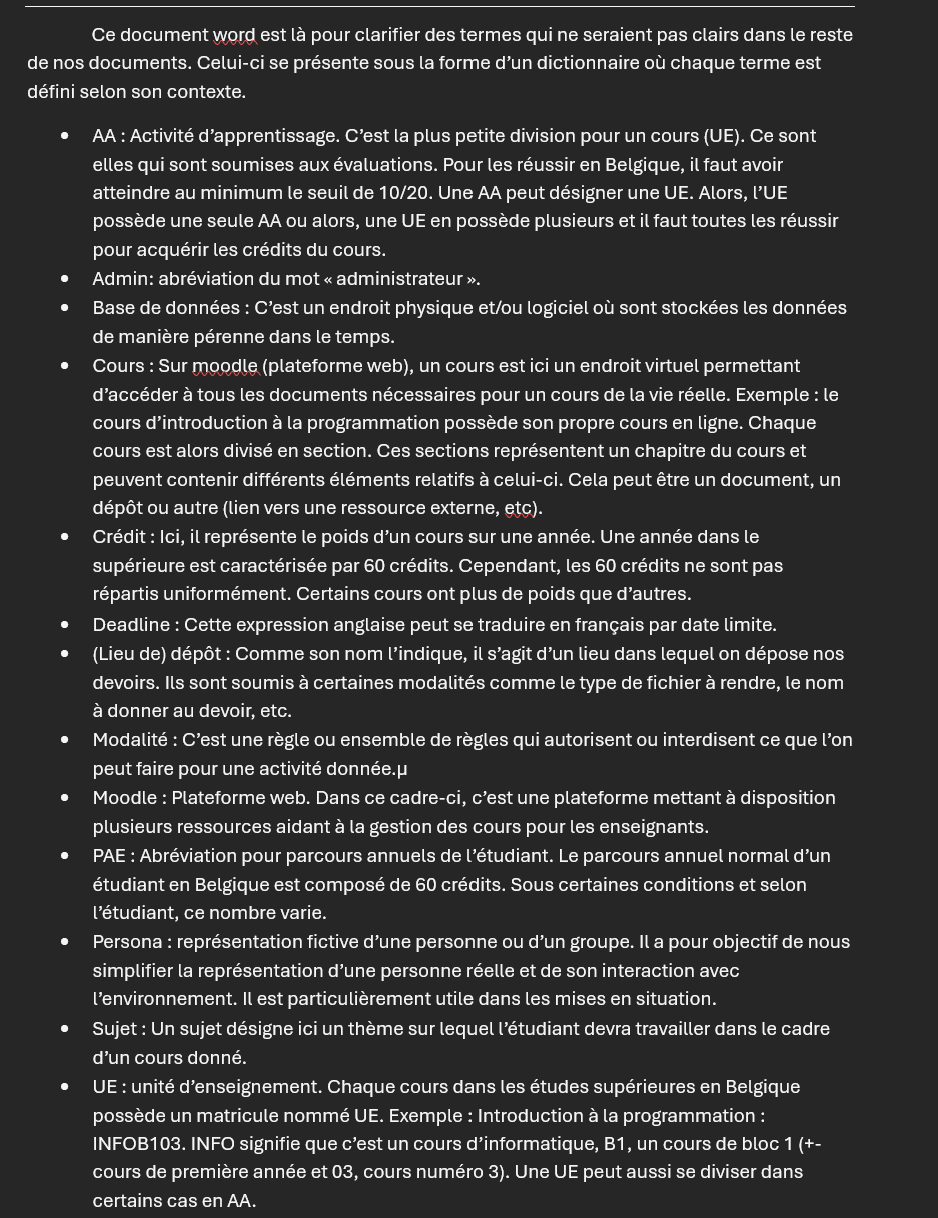
\includegraphics[width=2cm]{1.png}
                \caption{Lexique}
            \end{figure}

        \end{column}
    \end{columns}
\end{frame}


\end{document}